\section{Recommender Systems}
\label{sec:recommender}

A recommender systems is a powerful and versatile approach to user modeling.
Whenever we wish to predict the relevance of an item to a user, recommender systems are the tools to use.
Such systems are commonly used on the Web to provide a host of functionality, including:

\begin{itemize*}
  \item Suggesting new social connections based on an existing social graph.
  \item Recommending new and unseen products based on past purchases.
  \item Ordering news articles by predicted individual relevance.
  \item Recommending items based the activity of similar or like-minded users.
  \item Personalizing search results based on the current user's preferences.
\end{itemize*}

Note that although we use "ratings", "utility", "preference", "relevance" and "connection strength" depending on the context, 
they all basically mean the same, depending on the context. 
The terms are measures for what a user thinks of an item, using the domain language of the application in question.
These measures can be explicitly provided by each user, or implicitly mined from observed user behavior.

Common to our examples are a set of users, a set of items, and a sparse set of known ratings or relevance measures.
The operations of a recommender system is best described through graph operations, 
although the underlying algorithms might not use this as the representation at all.
\cite{Mirza2003} explain how any RS can be expressed as a graph traversal algorithm.
In this graph structure, items and users are nodes, while ratings, social connections et cetera are edges between the nodes.
An RS performs predictive reasoning by estimating the strengths of hypothetical connections between nodes that are not explicitly connected.

For example, if a user has rated a subset of the movies in a movie recommendation system, 
algorithms can use these ratings to predict how well the user will like unseen movies.
This inference can for instance be based on each movie's ratings from similar users.
In social networks, recommender systems can be used to infer new social relations 
based on existing connections. The principle is the same: By evaluating current explicit
connections, and the connections of similar users, new connections can be predicted.

As evident by the examples, recommender systems are powerful methods for user modeling, personalization and for fighting information overload.
Their ability to infer unknown relevance between users and items makes them useful in many situations, as we shall soon see.


\subsection{Interface Autonomy}

\begin{figure}[t]
  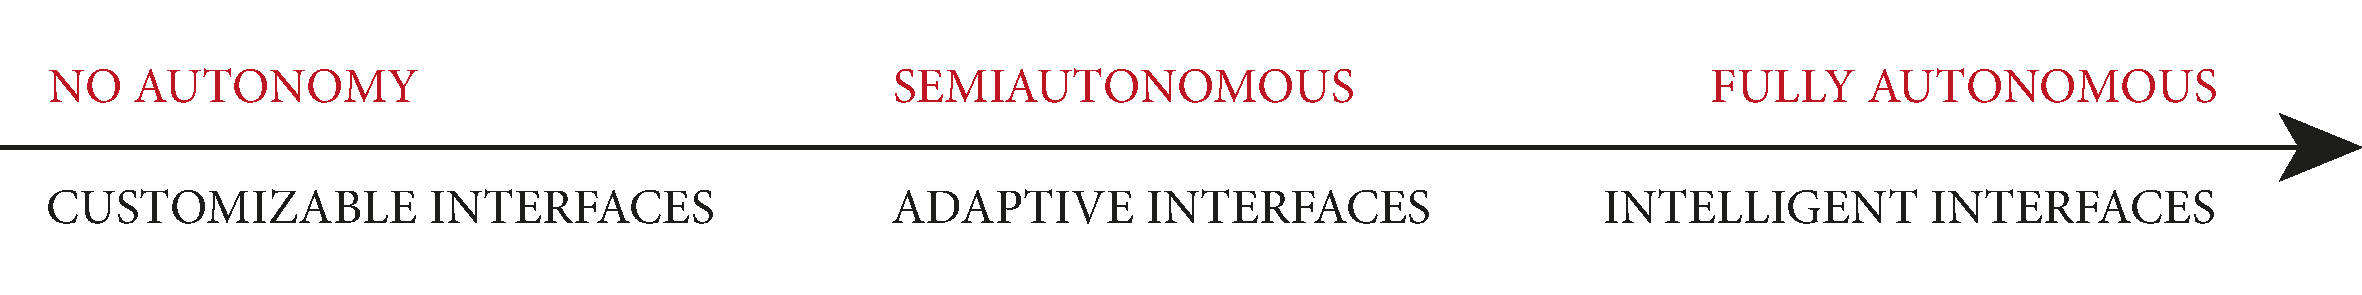
\includegraphics[width=\textwidth]{../graphics/autonomy.pdf}
  \caption[Levels of Interface Autonomy]{
    Levels of Interface Autonomy:
    Interfaces range from those only customizable by the user, 
    to intelligent systems takes the initiative on their own accord.
  }
  \label{fig:autonomy}
\end{figure}

Using AI to adapt an interface raises important questions with regard to usability, privacy and usefulness.
These questions are rooted in the autonomy expressed by each interface.
An autonomous interface is one that takes initiatives on its own, regardless of whether the user has asked for it \cite[p2]{Lieberman}. 
Naturally, any application that automatically personalizes its content will be autonomous to some degree.

Adaptive interfaces can be classified into increasing order of autonomy (see Figure \ref{fig:autonomy}). 
At the order of least autonomous systems, we have \emph{customizable interfaces}. 
These are interfaces that the user may customize themselves, but that do not take the initiative or change anything without explicit user action. 
For example, an interface might have a settings panel where users can change the order of items in a menu.
At the next level of autonomy, we have \emph{adaptive interfaces} that suggest to the user possible changes or actions that might be beneficial. For example, an email application could suggest which folder an email should be moved to.
At the most autonomous level, \emph{intelligent interfaces} implicitly and automatically customize the interface or content based on passive observation of the user. 
This could for instance entail automatic filing of emails based on content classification and data mining of previous user actions with similar messages.

An application that personalizes content automatically will fall somewhere in the two last categories and present either an adaptive or intelligent interface, 
depending on the extent and transparency of its autonomy.
In this thesis, we are only interested in fully autonomous, intelligent interfaces.
We wish to create a system that implicitly, and without any effort from each user,
can adapt the content of an application based on previous behavior
Examples of such implicit user modeling include \cite{Qiu2006}, \cite{Shen2005} and \cite{Carmel2009}.


\subsection{Aspects of Recommender Systems}

Formally, a recommender system can be seen as a quintuple, 
$\mathrm{RS} = (I, U, R, F, M)$,
where 
$I$ is the set of items and 
$U$ is the set of users.
$R$ is the set of known ratings or utility, for example explicit preferences given by users for certain items, or connections in a social graph.
We have explicit ratings whenever the user provides their own ratings (e.g. product purchases),
and implicit ratings when the system infers ratings from behavior (e.g. query log mining).
$F$ is a framework for representing the items, users and ratings, for example with a graph or matrix. 
$M$ is the actual user modeling algorithm used to infer unknown ratings 
for predicting a user's preference for an unrated item. This is where AI comes in.

In \citet[p2]{Adomavicius2005}, $M$ is seen as a utility (the rating, in AI terms) estimation function
$p: U \times I \rightarrow S$. Here, $p$ (for prediction) is a function that maps the set
of users and items into a fully ordered set of items $S$, ranked by their
utility to each user. In other words, $S$ is the completely specified version of $R$,
where each user has either an explicit, implicit or predicted preference for each item in $I$.
To predict the most relevant unrated item for each user, we simply find the item with the highest expected utility:

\begin{eqsp}
  \forall u \in U,\text{ } i'_u = \arg\max_{i \in I} p(u,i)
\end{eqsp}

The utility function $p$ depends on the modeling method being used, the active user and the item in question. 
The \emph{reason} for using a recommender system is that the utility is not defined for the entire $U \times I$ space, 
that is, the system does not know the utility of each item for each user. 
The point of a recommender system is then to extrapolate $R$ to cover the entire user-item space. 
In other words, to be able to rank items according to user preferences, 
the system must be able to predict each user's reaction to items they have not yet explicitly or implicitly rated themselves. 

Another common way of describing and implementing an RS is using a simple matrix.
This is what we shall use in this thesis. 
In this matrix, one dimension represents users and the other represents items.
Each populated cell corresponds to a known rating. 
This matrix corresponds to the framework variable $F$ in our RS quintuple:

\begin{eqsp}
 R_{u,i} =
 \begin{pmatrix}
  r_{1,1} & r_{1,2} & \cdots & r_{1,i} \\
  r_{2,1} & r_{2,2} & \cdots & r_{2,i} \\
  \vdots  & \vdots  & \ddots & \vdots  \\
  r_{u,1} & r_{u,2} & \cdots & r_{u,i}
 \end{pmatrix}
\end{eqsp}
%
Critically, these matrices are usually extremely sparse (most of the cells are empty). 
While there may be a large number of users and items, each individual user
only rates, connects to or uses a few of items.
This is true for any scenario where users explicitly rate items, access items in search results,
or connect to each other in a social network. 
For example, in the seminal Netflix Challenge movie recommender dataset, almost 99\% of the potential
user/item pairs have no rating \cite[p1]{Bell2007d}. In other words, 
this recommender system had to be able to produce results from a matrix where only 1\% of the cells had meaningful values.

This is often the defining characteristic of a recommender system: 
its ability to extract meaningful patterns from sparse data, 
through dimensionality reduction, neighborhood estimation and many other methods, as we shall soon see.
Naturally, much research looks at ways to best tackle this sparsity problem
(e.g. \cite{Pitsilis2009}, \citet[p3]{Claypool1999}, \citet[p19]{Ziegler2005}).

Recommender systems face many challenges other than this sparsity problem.
A directly related problem is the need for large datasets. Since the data is often sparse,
the systems will most often perform well if used on large numbers of items and users.
In addition, as in many machine learning methods, concept drift \cite[p1]{Widmer1996}, 
where the characteristics of a user or item
changes over time, is another recurring problem.

Another potential problem is that the performance of RSs is often closely tied to their computational complexity
(as mentioned in \citet[p6]{Adomavicius2005}). 
Real world usage of the most precise methods can be hindered by the computational power needed to actually put them into production.

Finally, the scale of the data in question should be a concern. If the ratings are ordinal data (e.g. 1-5)
input directly by users, the RS should take into account the domain specific meaning of these intervals.
For example, in a system for rating movies, the jump between ratings 4-5 might not have the same significance as
the jump from 2-3. However, this is a fact seldom mentioned in the literature. Most RSs 
employ metrics that assume a normal distribution, and even the common
evaluation techniques such as RMSE or MAE treat ordinal data as a continuous scale.
We will get back to these problems in Chapters \ref{chap:results} \emph{\&} \ref{chap:discussion}. 
% http://technocalifornia.blogspot.com/2011/04/recommender-systems-were-doing-it-all.html


\subsection{Predicting Ratings}

The crucial part of any RS is how it predicts unknown ratings.
Because of this, each method may be categorized based on certain dimensions of its predictive capabilities (see Table \ref{table:taxonomy}).
In this thesis, we use a taxonomy where these dimensions are: 
(1) the available \emph{data}, 
(2) the prediction \emph{method}, 
(3) the model \emph{granularity}, 
(4) the knowledge \emph{temporality} and 
(5) the knowledge gathering \emph{agents}.

\begin{table}[b]
  \begin{tabular*}{\textwidth}{ p{3cm} l @{\extracolsep{\fill}} }
    \toprule
    \emph{Variable} & \emph{Possible values} \\
    \midrule
    Data & Content-based | Collaborative | Hybrid\\
    Method & Heuristic | Model-based\\
    Granularity & Canonical | Typical | Individual\\
    Temporality & Short-term | Long-term\\
    Agents & Implicit | Explicit\\
    \bottomrule
  \end{tabular*}
  \caption[Recommender Systems Taxonomy]{A taxonomy of recommender systems. From \cite{Bjorkoy2010d}.}
  \label{table:taxonomy}
\end{table}

(1) The \emph{data} variable represents what data an RS uses to perform predictions. 
\emph{Content-Based} (CB) methods use only items, intra-item relations, and 
an individual user's past history as predictive signals of future actions \cite[p1]{Pazzani2007}.
By only considering the individual user in adapting an application, highly personal models can be created. 
However, such methods may require a lot of interaction before reliable models can be created \cite[p4]{Adomavicius2005}.
The problem of having to do complex inference from little data, as it often is in content-based predictions,
similar to the \emph{sparsity problem}, is often called the \emph{cold start} or \emph{new user} problem. 
This is closely related to the common AI problem of \emph{overfitting} data, 
where the algorithms creates models that match the training data, 
but not the actual underlying relationships. 
As with the sparsity problem, a lot of research looks at ways to overcome sparse data, i.e. achieving "warmer" cold start
(e.g. \cite{Said2009}, \cite{Lilegraven2011}). 
Formally, when using content-based predictions, the utility function $p(u,i)$ of user $u$ and item $i$ is extrapolated from $p(u,i_x)$, 
where $i_x$ is an item similar to $i$ and $p(u,i_x)$ is known \cite[p2]{Adomavicius2005}.

\emph{Collaborative Filtering} (CF) methods build predictive models for users based on the actions of similar users \citep{Schafer2007}.
The key observation is that similar users should have similar usage and action patterns. 
By using data from more than one user, expansive models that rely on actual user preferences may be built. 
These methods are especially useful when considering new users arriving in a system. 
A central problem with collaborative methods is that the resulting model is not as individually tailored as one created through content-based prediction. 
Collaborative models must be careful not to represent the \emph{average} user, but a single individual.
Formally, when using a collaborative method, 
the utility $p(u,i)$ of item $i$ for user $u$ is extrapolated from the known $p(u_x,i)$ where $u_x$ is a user similar to $u$
\cite[p4]{Adomavicius2005}. 

Because of \emph{the new user problem} of content-based prediction and the \emph{average user problem} of collaborative prediction, 
many systems use a hybrid approach (as introduced by \cite{Burke2007}).
By combining content-based and collaborative methods, 
systems that properly handle predictions for new users and avoid too much generalization in the models can be achieved. 
We will discuss hybrid aggregation systems later in this chapter.

(2) The \emph{method} variable is another way to classify recommenders. Orthogonal to what data the method uses, this variable
concerns \emph{how} the data is used.
First, we have the \emph{model-based} approach, where the recommender system builds predictive models based on the known data. 
Unseen items can then be fed into this model to compute its estimated utility score
\cite[p5]{Adomavicius2005}. 
For example, creating a Bayesian networks from past interaction is a model-based approach.

The other category is the \emph{heuristic} or \emph{memory-based} approach \cite[p5]{Adomavicius2005}. 
These methods use the raw data of items, users and ratings to directly estimate unknown utility values. 
For example, recommending items similar to the ones already rated by computing the cosine similarity of their feature vectors is a heuristic approach.

(3) The \emph{granularity} variable tells whether this approach creates models for the canonical user, stereotypical users or individual users. 
The canonical user is another term for the \emph{average} user, indicative of systems that adapt by seeing all users as a single entity. 
Stereotypical systems look at groups of users. 
For example, \cite{Rich1979} presented one of the first user modeling systems based on stereotypes, 
used to predict which books in a library each user would most enjoy.
Here, a dialogue between the system and the user was performed to place the user into a set of stereotypes. 
Each stereotype has a set of \emph{facets} which is then used to match books and users.
This created user models of \emph{typical} granularity, as opposed to common \emph{individual} approaches.

(4) \emph{Temporality} refers to how volatile the gathered knowledge will be.
While most RSs produce long term, relatively stable knowledge based on lasting user preference and taste, 
some systems use fluctuating parameters such as the time of day, exact location and the current context to produce recommendations.
For example, \cite{Horvitz} used clues from a user's calendar, camera and other sensors to determine the attentional state
of the user before delivering personalized and contextual notifications.

(5) The \emph{agents} variable signifies whether the knowledge gathering and presentation is implicit and opaque, 
or explicit and requires dedicated user interaction. Explicit feedback through ratings is 
common in movie, product or music rating services (e.g. \cite{Bell2007, Basu1998, Hotho}). 
However, for other services such as personalized search,
implicit mining of query logs and user interaction is often used to build predictive models 
(e.g. \cite{Shen2005, Agichtein2006, Speretta2000, Teevan2005}).



